\Subsection{7.3 Скручивание и поворот с помощью ROS}


ROS использует тип сообщения \href{http://www.ros.org/doc/api/geometry_msgs/html/msg/Twist.html}{Twist} (см. Подробности ниже) для публикации команд движения, которые будут использоваться базовым контроллером. Хотя для темы можно использовать практически любое имя, обычно оно называется / cmd\_vel, что сокращенно от «скорости команд». Узел базового контроллера подписывается на тему / cmd\_vel и преобразует сообщения Twist в сигналы двигателя, которые фактически вращают колеса. 

Чтобы увидеть компоненты сообщения Twist, выполните команду:

```text
$ rosmsg show geometry_msgs/Twist
```

который даст следующий результат:



> ```text
> geometry_msgs/Vector3 linear
>   float64 x
>   float64 y
>   float64 z
>   geometry_msgs/Vector3 angular
>   float64 x
>   float64 y
>   float64 z
> ```

Как видите, сообщение Twist состоит из двух вложенных сообщений с типом Vector3, одно для компонентов линейной скорости x, y и z, а другое для компонентов угловой скорости x, y и z. Линейные скорости указаны в метрах в секунду, а угловые скорости - в радианах в секунду. (1 радиан равен приблизительно 57 градусам.) 

Для робота с дифференциальным приводом, работающего в двухмерной плоскости (такой как пол), нам нужны только линейный компонент x и угловой компонент z. Это потому, что этот тип робота может двигаться только вперед / назад вдоль своей продольной оси и вращаться только вокруг своей вертикальной оси. Другими словами, линейные компоненты y и z всегда равны нулю (робот не может двигаться вбок или вертикально), а угловые компоненты x и y всегда равны нулю, поскольку робот не может вращаться вокруг этих осей. Всенаправленный робот также будет использовать линейный компонент y, в то время как летающий или подводный робот будет использовать все шесть компонентов.

#### _\textbf{7.3.1 Пример твист-сообщений}_

 Предположим, мы хотим, чтобы робот двигался прямо со скоростью 0,1 метра в секунду. Это должно потребовать двустороннего сообщения с линейными значениями x = 0,1, y = 0 и z = 0, а угловые значения x = 0, y = 0 и z = 0. Если вы укажете это сообщение в командной строке, часть сообщения будет иметь вид:

> '{linear: {x: 0.1, y: 0, z: 0}, angular: {x: 0, y: 0, z: 0}}'

Обратите внимание на то, как мы разграничиваем под-сообщения с помощью фигурных скобок и отделяем имена компонентов от их значений двоеточием и пробелом (пробел необходим!) Хотя это может показаться много печатанием, таким способом мы редко будем управлять роботом. Как мы увидим позже, сообщения Twist будут отправляться роботу с использованием других узлов ROS. 

Чтобы повернуть против часовой стрелки с угловой скоростью 1,0 радиан в секунду, требуемое сообщение Твист будет:

> '{linear: {x: 0, y: 0, z: 0}, angular: {x: 0, y: 0, z: 1.0}}'

 Если бы мы объединили эти два сообщения, робот двинулся бы вперед, повернувшись влево. TheresultingTwistmessagewouldbe:

> '{linear: {x: 0.1, y: 0, z: 0}, angular: {x: 0, y: 0, z: 1.0}}'

 Чем больше угловое значение z по сравнению с линейным значением x, тем сильнее поворот.

7.3.2 Мониторинг движения робота с помощью RViz 

Мы будем использовать RViz для визуализации движения робота, когда будем пробовать различные команды Twist и сценарии управления движением. Вспомните из \href{http://docs.ros.org/indigo/api/rviz/html/user_guide/}{Руководства пользователя RViz}, что мы можем использовать тип отображения \href{http://wiki.ros.org/rviz/DisplayTypes/Odometry}{одометрии}, чтобы отслеживать позу (положение и ориентацию) робота в различных точках его пути. Каждая поза робота обозначена большой стрелкой, указывающей в направлении, в котором робот находился в этой точке. Обратите внимание, что эти позы отражают то, что сообщается одометрией робота, которая может отличаться - иногда существенно - от того, как робот позиционируется в реальном мире. Однако, если робот хорошо откалиброван и работает на относительно твердой поверхности, данные одометрии обычно достаточно хороши, чтобы получить приблизительное представление о том, как работает робот. Кроме того, при запуске искусственного робота в симуляторе ArbotiX, где нет физики, соответствие будет точным. 

Давайте попробуем пару примеров с использованием симулятора ArbotiX. Сначала запустите поддельный TurtleBot с помощью команды:

```text
$ roslaunch rbx1_bringup fake_turtlebot.launch
```

В другом терминале вызовите RViz с уже включенным файлом конфигурации с дисплеем Одометрия: 

```text
$ rosrun rviz rviz -d `rospack find rbx1_nav`/sim.rviz
```

Наконец, откройте еще одно окно терминала и установите робота, движущегося по кругу по часовой стрелке, опубликовав следующее сообщение Twist: 

```text
$ rostopic pub -r 10 /cmd_vel geometry_msgs/Twist '{linear: {x: 0.1, y: 0, z: 0}, angular: {x: 0, y: 0, z: -0.5}}'
```

Мы используем параметр -r для постоянной публикации сообщений об ошибке на частоте 10 Гц. Некоторые роботы, такие как TurtleBot, требуют, чтобы команда движения постоянно публиковалась, иначе робот остановится: хорошая функция безопасности. Хотя этот параметр не является обязательным при запуске симулятора ArbotiX, он также не повредит. 

Если все работает нормально, результат в RViz должен выглядеть примерно так:

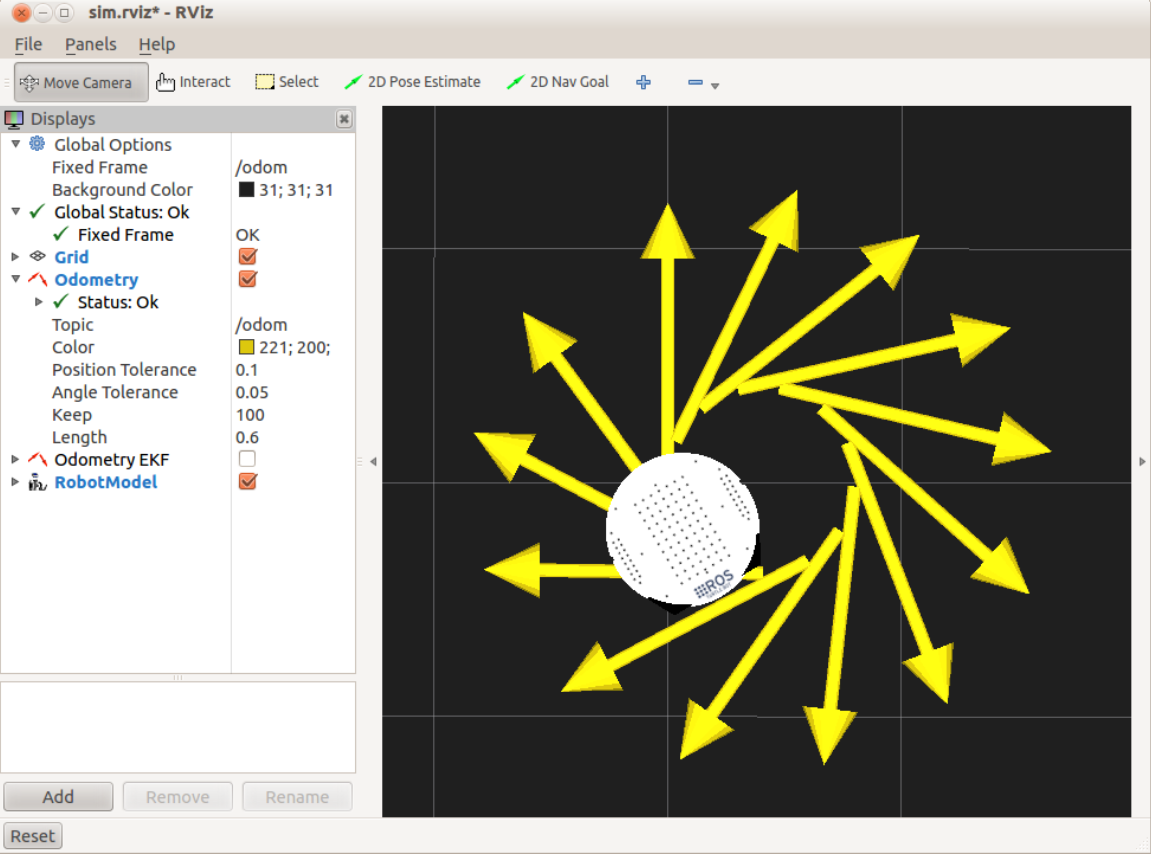
\includegraphics[width=9cm]{.gitbook/assets/snimok-ekrana-2020-05-30-v-13.44.51.png}

Обратите внимание, что мы установили в поле \textbf{Keep} значение 100 для отображения \textbf{одометрии}, которое указывает, что мы хотим отображать до 100 последних стрелок, прежде чем самая старая из них выпадет. \textbf{Допуск положения} (в метрах) и \textbf{допуск угла} (в радианах) позволяют вам контролировать частоту отображения новой стрелки. 

Чтобы убрать стрелки в любой точке, либо нажмите кнопку \textbf{«Сброс»}, либо снимите флажок рядом с дисплеем \textbf{«Одометрия»}, а затем снова проверьте его. Чтобы полностью отключить стрелки, не устанавливайте флажок.

 Чтобы остановить вращение робота, введите Ctrl-C в том же окне терминала, а затем опубликуйте пустое сообщение Twist:

```text
$ rostopic pub -1 /cmd_vel geometry_msgs/Twist '{}'
```

Теперь давайте попробуем второй пример. Сначала очистите стрелки одометрии, нажав кнопку \textbf{«Сброс»} в RViz. Следующая пара команд (разделенных точкой с запятой) будет сначала двигать робота прямо в течение примерно 3 секунд (опция «-1» означает «опубликовать один раз»), а затем продолжать бесконечно по кругу против часовой стрелки:

```text
$ rostopic pub -1 /cmd_vel geometry_msgs/Twist '{linear: {x: 0.2, y: 0, z: 0}, angular: {x: 0, y: 0, z: 0}}'; rostopic pub -r 10 /cmd_vel geometry_msgs/Twist '{linear: {x: 0.2, y: 0, z: 0}, angular: {x: 0, y: 0, z: 0.5}}'
```

Чтобы остановить робота, введите Ctrl-C в том же окне терминала и опубликуйте пустое сообщение Twist: 

```text
$ rostopic pub -1 /cmd_vel geometry_msgs/Twist '{}'
```

Прежде чем мы попробуем несколько сообщений Twist на реальном роботе, нам нужно обговорить некоторые моменты, говорящие о калибровке.

